%        File: WeeklyResearchReport_4_19_21.tex
%     Created: Mon Apr 19 08:00 AM 2021 E
% Last Change: Mon Apr 19 08:00 AM 2021 E
%
\documentclass[a4paper]{article}
\usepackage{mathtools}
\usepackage{verbatim}
\usepackage{graphicx}
\usepackage{tabularx}
\usepackage{pgfplots}
\usepackage{adjustbox}
\usepackage{booktabs}
\makeatletter
\let\latex@xfloat=\@xfloat
\def\@xfloat #1[#2]{%
    \latex@xfloat #1[#2]%
    \def\baselinestretch{1}
    \@normalsize\normalsize
    \normalsize
}
\makeatother
\usepackage{amsmath}
\usepackage{mathtools}
\usepackage{epigraph}
\usepackage{cancel}
\usepackage{xcolor}
\newcommand\Ccancel[2][black]{\renewcommand\CancelColor{\color{#1}}\cancel{#2}}
\usepackage{algorithm}
\usepackage{graphicx}
\usepackage[noend]{algpseudocode}
\usepackage{gnuplot-lua-tikz}
\usepackage[utf8]{inputenc}
\usepackage{pgfplots}
\usepackage{tabularx}
\usepackage{hyperref}
\DeclareUnicodeCharacter{2212}{−}
\usepgfplotslibrary{groupplots,dateplot}
\usetikzlibrary{patterns,shapes.arrows}
\pgfplotsset{compat=newest}
\begin{document}
\begin{titlepage}

    \title{
    Daily Research Report}

    \author{ Jeffrey Severino \\
        University of Toledo \\
        Toledo, OH  43606 \\
    email: jseveri@rockets.utoledo.edu}


    \maketitle

\end{titlepage}
\section{Current Research Direction}
\section{Research Performed}

\subsection{Results}

Hypothesis 1: 

By using a composite trapezoidal rule numerical integration technique, the speed
of sound is approximated using the tangential mach number. A second order 
convergence for the approximated speed of sound is expected (Refer to analysis). 
To obtain the radial derivatives, second and fourth order central differencing 
schemes were used and the order of accuracy will also be computed using the 
four system of equations for the LEE. 

Why is this my hypothesis?:
As the grid spacing gets smaller from one iteration to the next, the computed order of accuracy is
expected to approach a known value, which is the leading error term of the 
truncated term in the Taylor series used to derive the scheme , which in this
case is the composite trapezoidal rule. By using the MMS, a computed order
of accuracy was found. 



\begin{align}
       \bar{A} = \frac{\tanh{\left(\frac{r}{30} - \frac{1}{30} \right)}}{16} + \frac{\tanh{\left(\frac{r}{30} - \frac{11}{600} \right)}}{16} + \frac{\tanh{\left(\frac{r}{30} - \frac{1}{300} \right)}}{16} + \frac{709}{711} 
\end{align}


\begin{align}
     M_x = 0.5
\end{align}



\begin{align}
     0.177025756979167 \left(- \frac{0.333333333333333 r \tanh^{2}{\left(0.0333333333333333 r - 0.0333333333333333 \right)}}{\left(0.062676237268094 \tanh{\left(0.0333333333333333 r - 0.0333333333333333 \right)} + 0.062676237268094 \tanh{\left(0.0333333333333333 r - 0.0183333333333333 \right)} + 0.062676237268094 \tanh{\left(0.0333333333333333 r - 0.00333333333333333 \right)} + 1\right)^{1.0}} - \frac{0.333333333333333 r \tanh^{2}{\left(0.0333333333333333 r - 0.0183333333333333 \right)}}{\left(0.062676237268094 \tanh{\left(0.0333333333333333 r - 0.0333333333333333 \right)} + 0.062676237268094 \tanh{\left(0.0333333333333333 r - 0.0183333333333333 \right)} + 0.062676237268094 \tanh{\left(0.0333333333333333 r - 0.00333333333333333 \right)} + 1\right)^{1.0}} - \frac{0.333333333333333 r \tanh^{2}{\left(0.0333333333333333 r - 0.00333333333333333 \right)}}{\left(0.062676237268094 \tanh{\left(0.0333333333333333 r - 0.0333333333333333 \right)} + 0.062676237268094 \tanh{\left(0.0333333333333333 r - 0.0183333333333333 \right)} + 0.062676237268094 \tanh{\left(0.0333333333333333 r - 0.00333333333333333 \right)} + 1\right)^{1.0}} + \frac{r}{\left(0.062676237268094 \tanh{\left(0.0333333333333333 r - 0.0333333333333333 \right)} + 0.062676237268094 \tanh{\left(0.0333333333333333 r - 0.0183333333333333 \right)} + 0.062676237268094 \tanh{\left(0.0333333333333333 r - 0.00333333333333333 \right)} + 1\right)^{1.0}}\right)^{0.5}
\end{align}




The $L2_{norm}$ error of the two grids 
$\epsilon_{grid_i}$ and $\epsilon_{grid_i+1}$
\begin{figure}[!]
    \centering
    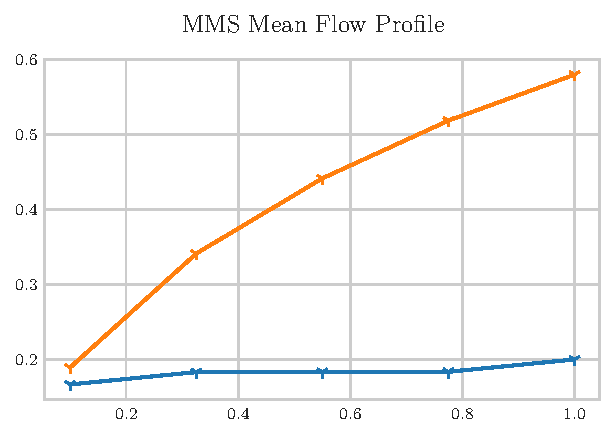
\includegraphics{/home/jeff-severino/SWIRL/CodeRun/03-plotReport/tex-outputs/MMS_mean_flow.pdf}
    \caption{The manufactured mean flow test case using a summation of Tangents for $A$ and $M_x$}
    \label{fig:1}
\end{figure}

\begin{figure}[!]
    \centering
    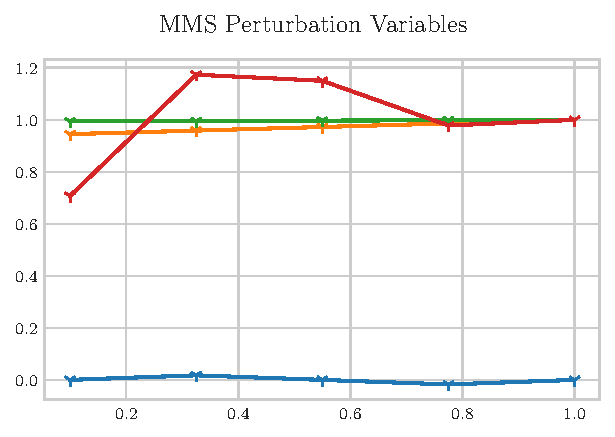
\includegraphics{/home/jeff-severino/SWIRL/CodeRun/03-plotReport/tex-outputs/MMS_perturbation_vars.pdf}
    \caption{The manufactured perturbation functions ,$v_r$, $v_x$, $v_{\theta}$, $p$}
    \label{fig:1a}
\end{figure}

\begin{figure}[!]
    \centering
    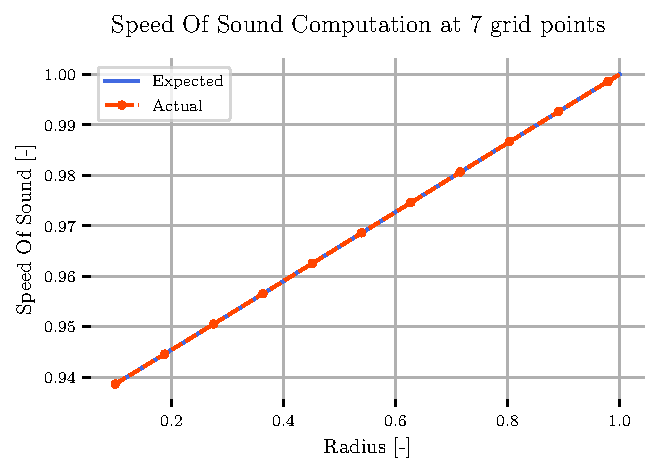
\includegraphics{/home/jeff-severino/SWIRL/CodeRun/03-plotReport/tex-outputs/SpeedOfSoundComparison1.pdf}
    \caption{}
    \label{fig:2}
\end{figure}



\begin{figure}[!]
    \centering
    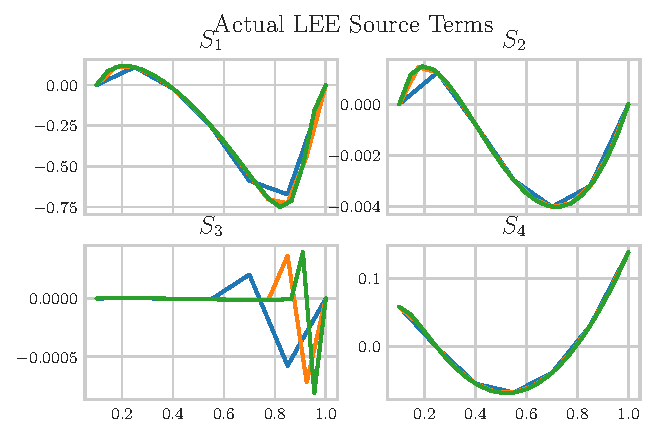
\includegraphics{/home/jeff-severino/SWIRL/CodeRun/03-plotReport/tex-outputs/SourceTermActual.pdf}
    \caption{}
    \label{fig:3}
\end{figure}


\begin{figure}[!]
    \centering
    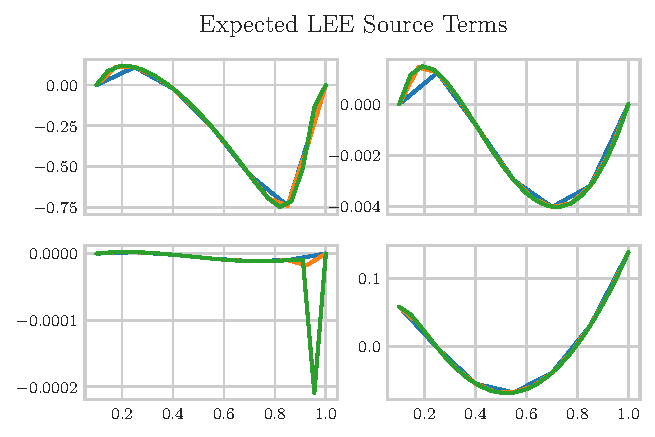
\includegraphics{/home/jeff-severino/SWIRL/CodeRun/03-plotReport/tex-outputs/SourceTermExpected.pdf}
    \caption{}
    \label{fig:3}
\end{figure}


\begin{figure}[!]
    \centering
    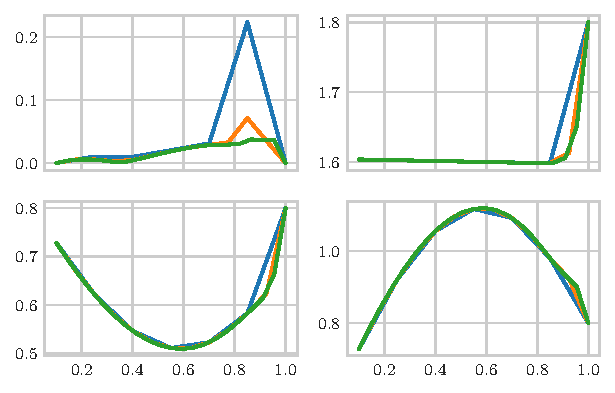
\includegraphics{/home/jeff-severino/SWIRL/CodeRun/03-plotReport/tex-outputs/SourceTermError.pdf}
    \caption{}
    \label{fig:3}
\end{figure}


\begin{figure}[!]
    \centering
    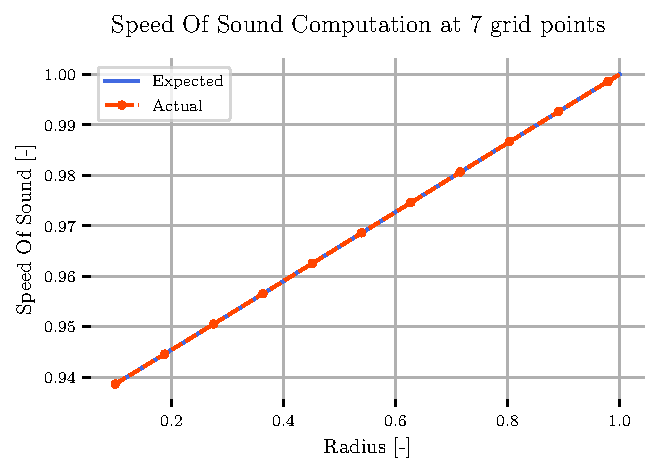
\includegraphics{/home/jeff-severino/SWIRL/CodeRun/03-plotReport/tex-outputs/SpeedOfSoundComparison1.pdf}
    \caption{}
    \label{fig:2}
\end{figure}


\begin{figure}[!]
    \centering
    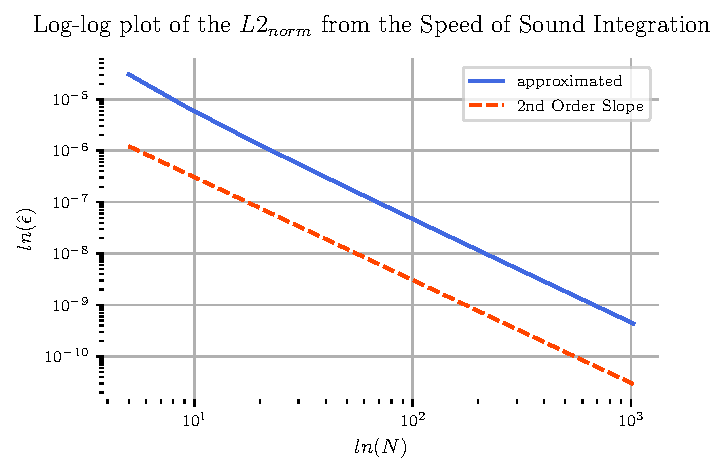
\includegraphics{/home/jeff-severino/SWIRL/CodeRun/03-plotReport/tex-outputs/SND_L2.pdf}
    \caption{}
    \label{fig:4}
\end{figure}


\begin{figure}[!]
    \centering
    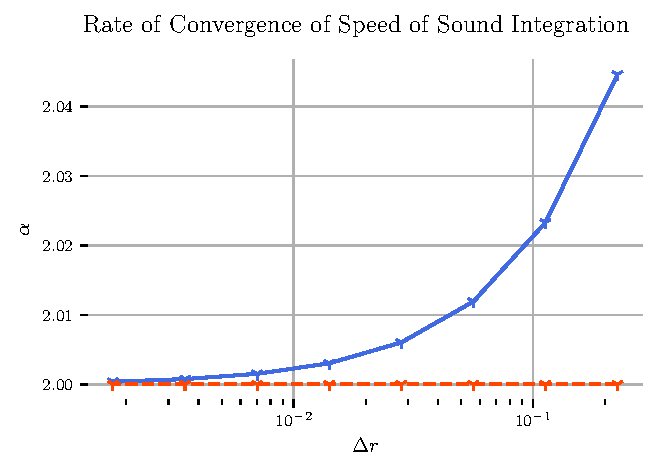
\includegraphics{/home/jeff-severino/SWIRL/CodeRun/03-plotReport/tex-outputs/SND_ROC.pdf}
    \caption{}
    \label{fig:5}
\end{figure}


\begin{figure}[!]
    \centering
    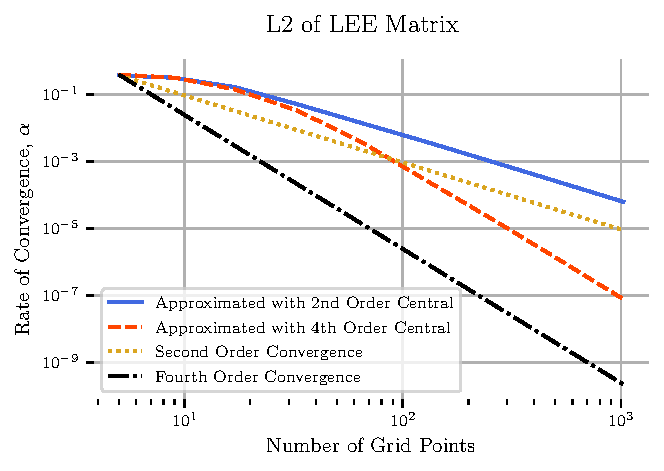
\includegraphics{/home/jeff-severino/SWIRL/CodeRun/03-plotReport/tex-outputs/LEE_L2.pdf}
    \caption{}
    \label{fig:6}
\end{figure}


\begin{figure}[!]
    \centering
        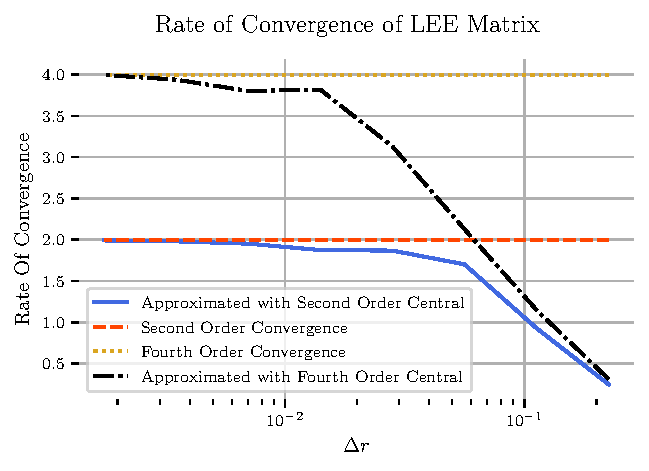
\includegraphics{/home/jeff-severino/SWIRL/CodeRun/03-plotReport/tex-outputs/LEE_ROC.pdf}
        \caption{}
        \label{fig:7}
\end{figure}





\section{Issues and Concerns}
I attempted at varying the grid aspect ratio but did not get better results.
I want to report the source term expressions.
\section{Planned Research}
Write results and discussion for these graphs.
\end{document}


